\chapter{Implementacija i korisničko sučelje}
		
		
		\section{Korištene tehnologije i alati}
		
			%\textbf{\textit{dio 2. revizije}}
			
			% \textit{Detaljno navesti sve tehnologije i alate koji su primijenjeni pri izradi dokumentacije i aplikacije. Ukratko ih opisati, te navesti njihovo značenje i mjesto primjene. Za svaki navedeni alat i tehnologiju je potrebno \textbf{navesti internet poveznicu} gdje se mogu preuzeti ili više saznati o njima}.
			{Komunikacija unutar grupe najviše se odvijala preko aplikacije \underline{Discord}\footnote{\url{https://discord.com/}}, a manjim dijelom u početku putem Microsoftove platforme za poslovnu komunikaciju \underline{Teams}\footnote{\url{https://www.microsoft.com/hr-hr/microsoft-teams/}}. Za izradu gotovo svih UML dijagrama korišten je alat \underline{Astah UML}\footnote{\url{https://astah.net/products/astah-uml/}}, dok je dijagram baze podataka napravljen uz pomoć razvojnog okruženja \underline{DataGrip}\footnote{\url{https://www.jetbrains.com/datagrip/}} tvrtke JetBrains. Upravljanje različitim verzijama koda i dokumentacije obavljanno je uz pomoć sustava \underline{Git}\footnote{\url{https://git-scm.com/}}, a podatci su se čuvali u udaljenom repozitoriju na platformi \underline{GitLab}\footnote{\url{https://gitlab.com/}}.}
			
			{Članovi tima koji su izrađivali \textit{backend} koristili su \underline{IntelliJ IDEA}\footnote{\url{https://www.jetbrains.com/idea/}} ili \underline{Eclipse}\footnote{\url{https://www.eclipse.org/}} kao razvojno okruženje, dok su članovi na \textit{frontendu} koristili \textit{editor} \underline{Visual Studio Code}\footnote{\url{https://code.visualstudio.com/}}. IntelliJ i Eclipse su razvojna okruženja primarno namijenjena za razvoj softvera u Javi; Eclipseova funkcionalnost može se znatno proširiti \textit{plug-inovima}. Visual Studio Code jednostavan je uređivač izvornog koda koji se može koristiti s raznim programskim jezicima, a razvio ga je Microsoft.}
			
			{Za izradu \textit{backenda} aplikacije korišteni su radni okvir \underline{Spring Boot}\footnote{\url{https://spring.io/projects/spring-boot}} i jezik \underline{Java}\footnote{\url{https://www.java.com/}}. Spring Boot je specijalizacija radnog okvira \underline{Spring}\footnote{\url{https://spring.io/projects/spring-framework}} (ne nadomješta Spring) koja pojednostavljuje oblikovanje web aplikacije jer automatski konfigurira važne funkcionalnosti Springa. Na \textit{frontend} strani aplikacije korišteni su \underline{React}\footnote{\url{https://reactjs.org/}} i \underline{JavaScript}\footnote{\url{https://www.javascript.com/}}. React tehnički nije radni okvir, nego knjižnica pisana u JavaScriptu, iako se smatra jednim od najznačajnijih \textit{frontend} radnih okvira u vrijeme izrade ovog projekta.}
			
			{Aplikacija je puštena u pogon na poslužitelju \underline{Heroku}\footnote{\url{https://www.heroku.com/}}, a baza podataka povezana je na Heroku preko \underline{Amazon AWS}\footnote{\url{https://aws.amazon.com/products/databases/}} usluge.}
			\eject 
		
	
		\section{Ispitivanje programskog rješenja}
			
%			\textbf{\textit{dio 2. revizije}}\\
%			
%			 \textit{U ovom poglavlju je potrebno opisati provedbu ispitivanja implementiranih funkcionalnosti na razini komponenti i na razini cijelog sustava s prikazom odabranih ispitnih slučajeva. Studenti trebaju ispitati temeljnu funkcionalnost i rubne uvjete.}
	
			
			\subsection{Ispitivanje komponenti}
%			\textit{Potrebno je provesti ispitivanje jedinica (engl. unit testing) nad razredima koji implementiraju temeljne funkcionalnosti. Razraditi \textbf{minimalno 6 ispitnih slučajeva} u kojima će se ispitati redovni slučajevi, rubni uvjeti te izazivanje pogreške (engl. exception throwing). Poželjno je stvoriti i ispitni slučaj koji koristi funkcionalnosti koje nisu implementirane. Potrebno je priložiti izvorni kôd svih ispitnih slučajeva te prikaz rezultata izvođenja ispita u razvojnom okruženju (prolaz/pad ispita). }

			{Ispitivanje komponenti provodimo pomoću JUnit javinog okvira za testiranje i pisanjem ispitnih slučajeva korištenjem jednog od javinih IDE, Eclipse ili IntelliJ.}
			
				\subsubsection {1. Ispitivanje traženja igrača korisničkim imenom}
				
					{Prilikom pisanja programskog koda za ovaj test koristi se anotacija \textit{@DataJpaTest} koji je specifičan za radni okvir \textit{spring} prilikom rada s \textit{Data Transfer Object} razredima. Očekivamo da će test biti uspješan i uspjeti pronaći igrača u bazi.}
					
						\begin{figure}[H]
							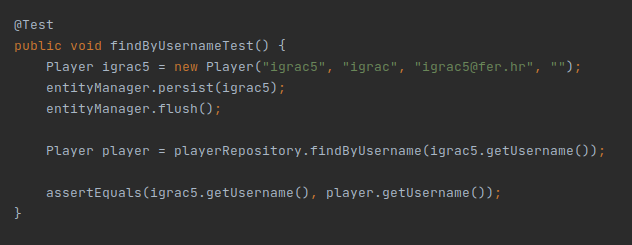
\includegraphics[width=\textwidth]{slike/playerFindByUsernameTest} 
							\centering
							\caption{Player Repository - JUnit, test}
							\label{}
						\end{figure}
					
				\subsubsection{Rezultat}
						
						\begin{figure}[H]
							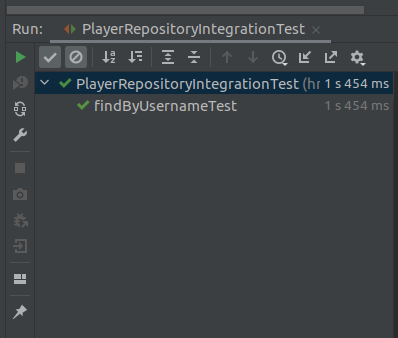
\includegraphics[width=\textwidth]{slike/playerFindByUsernameTest_result} 
							\centering
							\caption{Player Repository - JUnit, rezultat}
							\label{}
						\end{figure}
					
				\subsubsection {2. Ispitivanje traženja lokacije imenom}
				
					{Očekivamo da će test biti uspješan i uspjeti pronaći lokaciju u bazi.}
				
						\begin{figure}[H]
							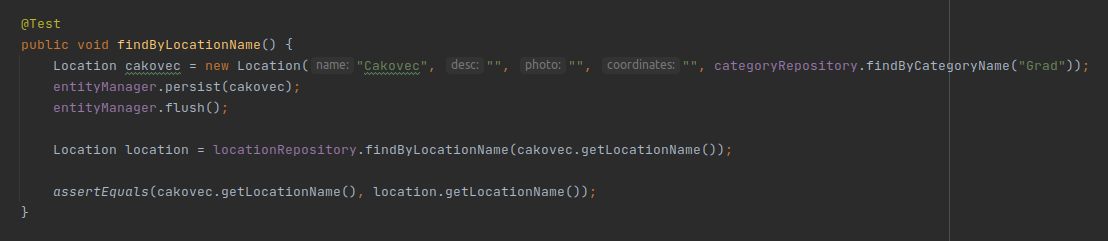
\includegraphics[width=\textwidth]{slike/locationFindByNameTest} 
							\centering
							\caption{Location Repository - JUnit, test}
							\label{}
						\end{figure}
					
				\subsubsection{Rezultat}
				
						\begin{figure}[H]
							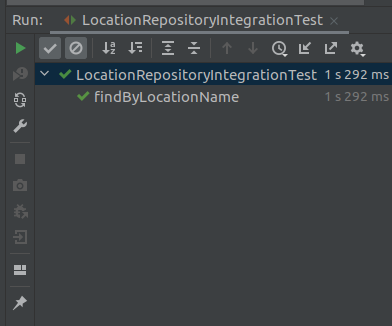
\includegraphics[width=\textwidth]{slike/locationFindByNameTest_result} 
							\centering
							\caption{Location Repository - JUnit, rezultat}
							\label{}
						\end{figure}
					
				\subsubsection {3. Ispitivanje traženja bespravnog zahtjeva za popis svih igrača}
					
					{Prilikom pisanja ovih testova koristi se anotacija \textit{@SpringBootTest} i \textit{@AutoConfigureMockMvc}. Očekivamo da će test biti uspješan jer se tijekom pretrage ne može obaviti provjera nad prijavljenim korisnikom kako bi se ustvrdilo da ima razinu adminstratorovih ovlasti.}
					
						\begin{figure}[H]
							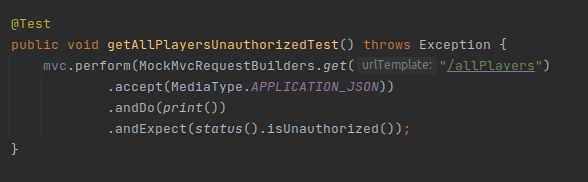
\includegraphics[width=\textwidth]{slike/unauthorizedTest} 
							\centering
							\caption{Admin Controller - JUnit, test}
							\label{}
						\end{figure}
					
				\subsubsection{Rezultat}
				
						\begin{figure}[H]
							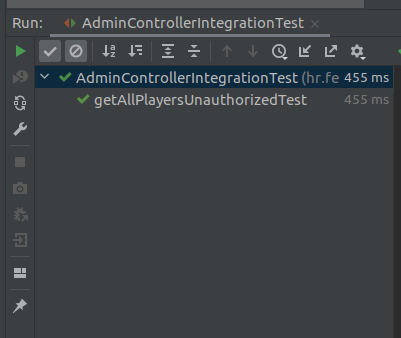
\includegraphics[width=\textwidth]{slike/unauthorizedTest_result} 
							\centering
							\caption{Admin Controller - JUnit, rezultat}
							\label{}
						\end{figure}
			
			\subsubsection {4. Ispitivanje razina ovlasti igrača i računanja udaljenosti}
			
				{Prilikom pisanja ovih testova koristi se anotacija \textit{@Mock} specifična za rad sa Service razredima. U ovom primjeru testiramo više metoda u razredu Player Service. Ispitujemo razine ovlasti kod postojećih igrača te metodu za računanje udaljenosti. Očekujemo da će za dane ulaze testovi proći.}
			
					\begin{figure}[H]
						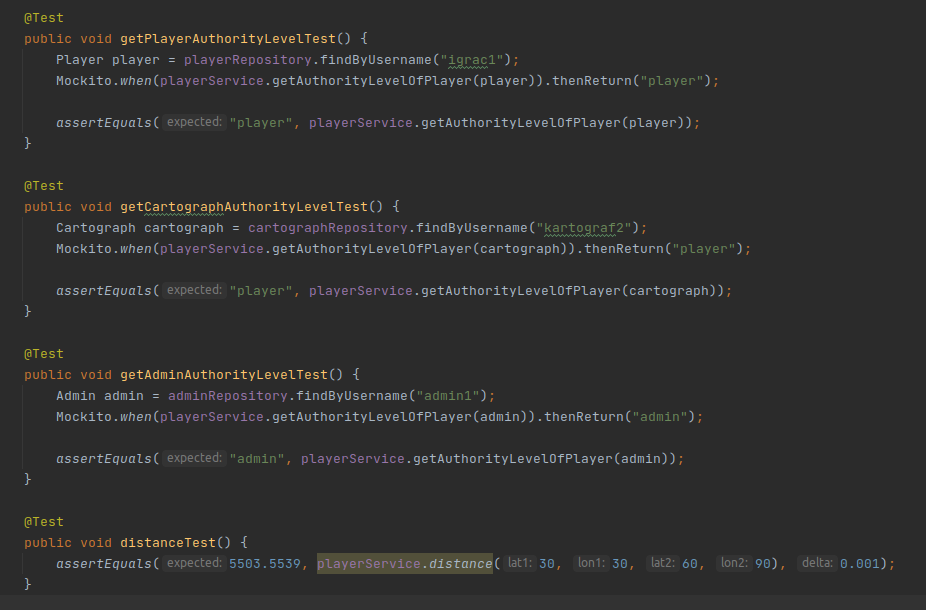
\includegraphics[width=\textwidth]{slike/playerServiceTest} 
						\centering
						\caption{Player Service - JUnit, test}
						\label{}
					\end{figure}
			
			\subsubsection{Rezultat}
			
					\begin{figure}[H]
						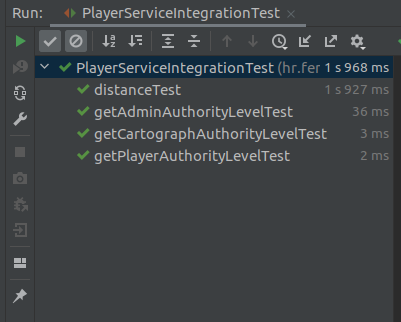
\includegraphics[width=\textwidth]{slike/playerServiceTest_result} 
						\centering
						\caption{Player Service - JUnit, rezultat}
						\label{}
					\end{figure}
			
			
			\eject
			
			\subsection{Ispitivanje sustava}
			
			% \textit{Potrebno je provesti i opisati ispitivanje sustava koristeći radni okvir Selenium\footnote{\url{https://www.seleniumhq.org/}}. Razraditi \textbf{minimalno 4 ispitna slučaja} u kojima će se ispitati redovni slučajevi, rubni uvjeti te poziv funkcionalnosti koja nije implementirana/izaziva pogrešku kako bi se vidjelo na koji način sustav reagira kada nešto nije u potpunosti ostvareno. Ispitni slučaj se treba sastojati od ulaza (npr. korisničko ime i lozinka), očekivanog izlaza ili rezultata, koraka ispitivanja i dobivenog izlaza ili rezultata.\\ }
			 
		%	 \textit{Izradu ispitnih slučajeva pomoću radnog okvira Selenium moguće je provesti pomoću jednog od sljedeća dva alata:}
		%	 \begin{itemize}
		%	 	\item \textit{dodatak za preglednik \textbf{Selenium IDE} - snimanje korisnikovih akcija radi automatskog ponavljanja ispita	}
		%	 	\item \textit{\textbf{Selenium WebDriver} - podrška za pisanje ispita u jezicima Java, C\#, PHP koristeći posebno programsko sučelje.}
		%	 \end{itemize}
		 %	\textit{Detalji o korištenju alata Selenium bit će prikazani na posebnom predavanju tijekom semestra.}
			
			{Ispitivanje sustava možemo provesti pomoću dodatka za preglednik Selenimu IDE i pisanjem ispitnih slučajeva korištenjem programskog sučelja, tj. mi koristimo Selenium WebDriver unutar JUnit testova. Pomoću dodatka za preglednik Selenium IDE snimaju se korisnikove akcije radi automatskog ponavljanja ispitnog slučaja.} 
			
			\subsubsection	{1. Ispitivanje dobre prijave na web aplikaciju GeoFighter }
			
				{Na ulazu unosimo podatke za prijavu već registriranog igrača (\emph{username: igrac1} i \emph{password: igrac}). Očekivani izlaz je preusmjeravanje na stranicu \emph{/home}. Preusmjeravanje pratimo prema elementima s određenih stranica. }
				
					\begin{figure}[H]
					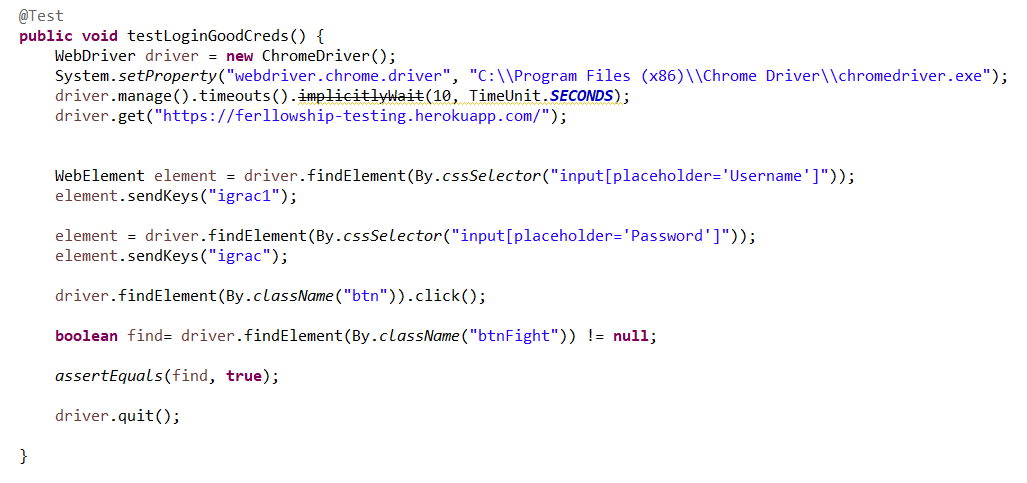
\includegraphics[width=\textwidth]{slike/JUSeTest1} 
					\centering
					\caption{Selenium WebDriver - JUnit, test1}
					\label{}
					\end{figure}
				
			\subsubsection{2. Ispitivanje loše prijave na web aplikaciju GeoFighter}
			
				{Na ulazu unosimo podatke za neregistriranog igrača (\emph{username: testadmin} i \emph{password: 22345}). Očekivani izlaz je ostanak na stranici za prijavu, što provjeravamo pomoću karakterističnih elemenata sa stranice.}
			
					\begin{figure}[H]
						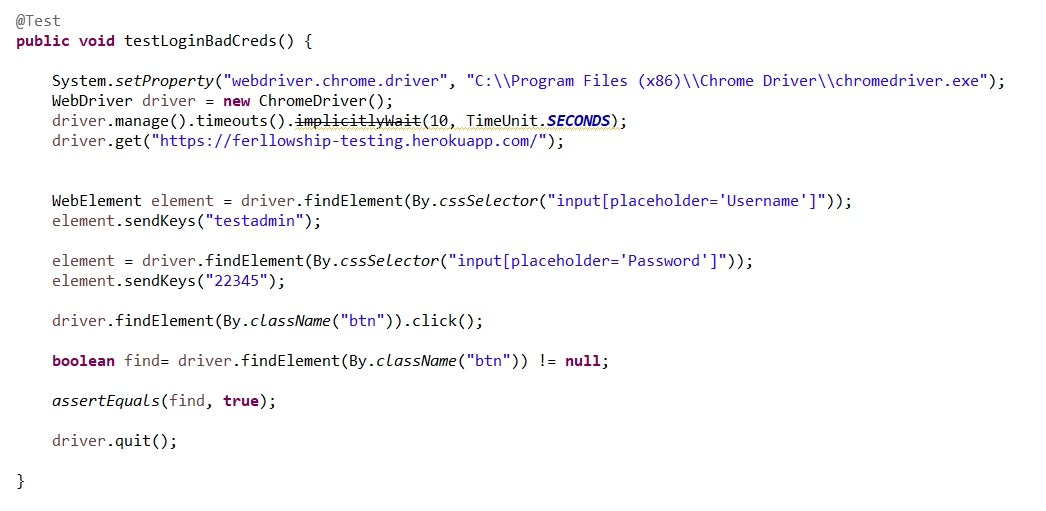
\includegraphics[width=\textwidth]{slike/JUSeTest2} 
						\centering
						\caption{Selenium WebDriver - JUnit, test2}
						\label{}
					\end{figure}
			
			\subsubsection{Rezultat}
			
				{Nakon pokretanja testova \emph{testLoginGoodCreds} i \emph{testLoginBadCreds}, dobili smo očekivani rezultat. Odnosno aplikacija je \textbf{prošla} testove.}
			
					\begin{figure}[H]
						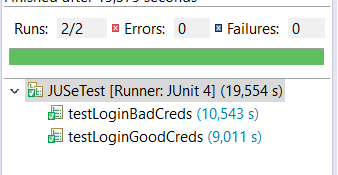
\includegraphics[width=\textwidth]{slike/rezultat_JUSeTest} 
						\centering
						\caption{Selenium WebDriver - JUnit, rezultat}
						\label{}
					\end{figure}
				
			\subsubsection{3. Ispitivanje postavljanja isključenja}
			
				{Ovo ispitvanje provodimo pomoću dodatka na Google Chrome \emph{Selenium IDE}. Prijavimo se kao \emph{admin1}, pregledamo profil \emph{igraca1}. Na ulazu testa unosimo trajno isključenje za \emph{igraca1} te se odjavimo kao \emph{admin1}. Očekivani izlaz je kad se pokušamo prijaviti kao \emph{igrac1} da nam to neće biti dozvoljeno dok će nam prijava kao \emph{igrac2} biti dozvoljena. Te radnje smo snimili pomoću Selenium IDE dodatka te ih pokrenuli s podatcima za \emph{igrac1}. Ako ponovno pokrenemo test i promijenimo korisničko ime na \emph{igrac2} vidimo da test dobro radi, odnosno s \emph{igrac2} smo se uspjeli prijaviti. Dobili smo željeni rezultat. Aplikacija je \textbf{prošla} test.}
					
					\begin{figure}[H]
						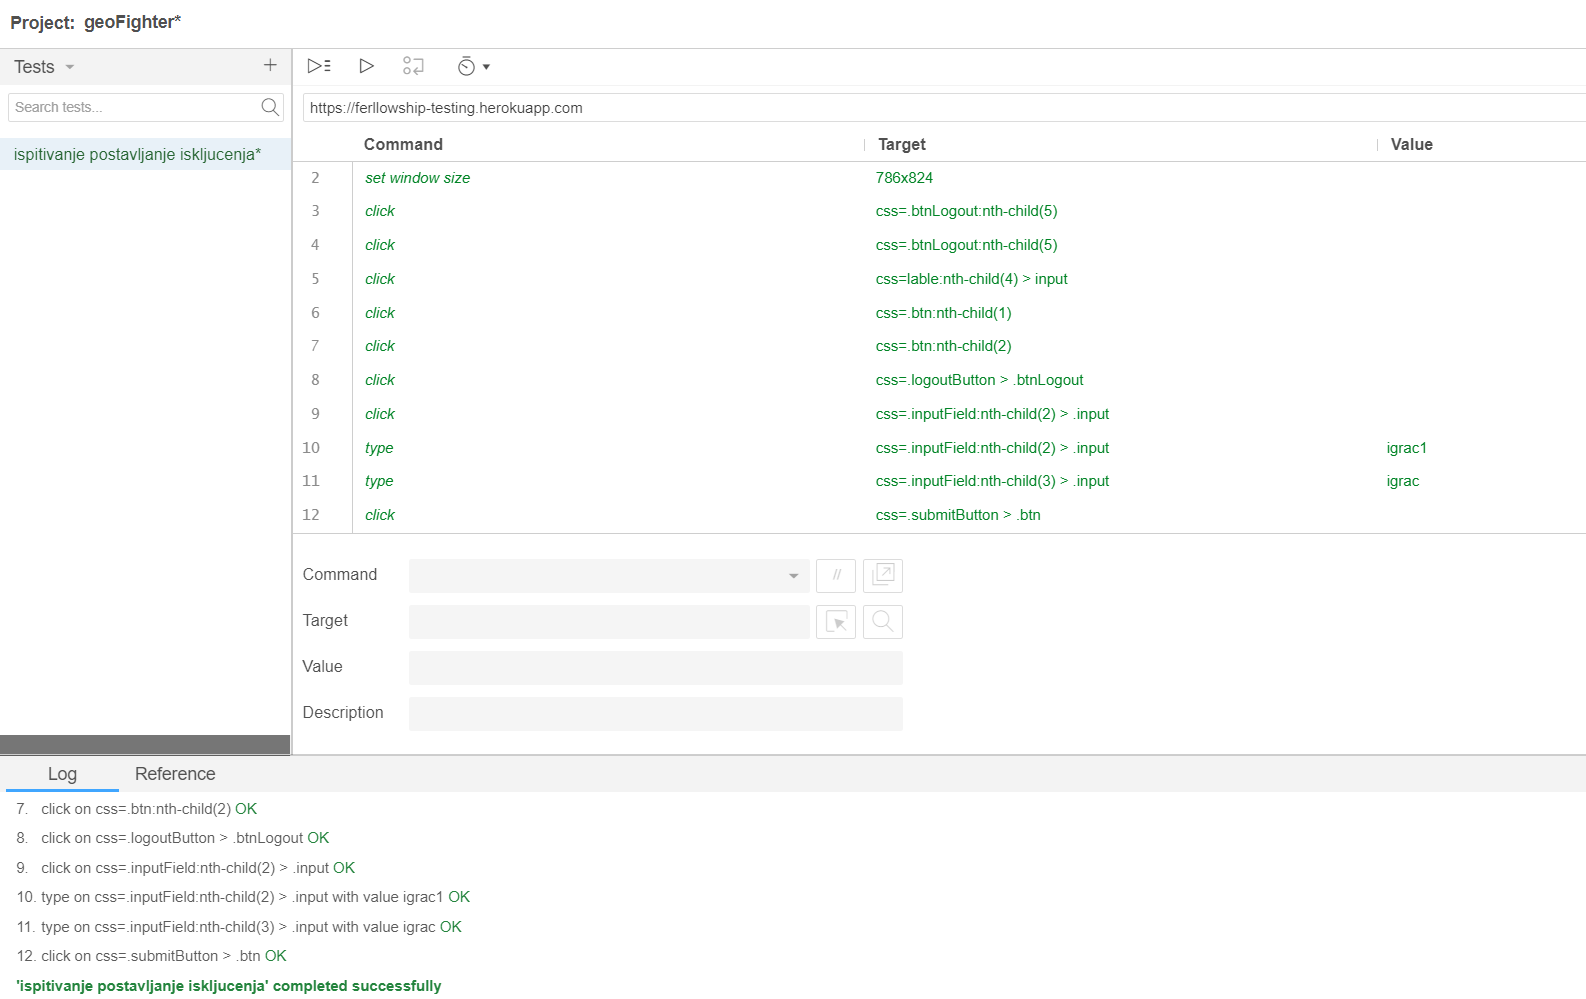
\includegraphics[width=\textwidth]{slike/SeleniumIDE_test1} 
						\centering
						\caption{Selenium IDE, ispitivanje postavljanja isključenja}
						\label{}
					\end{figure}
				\eject
			\subsubsection{4. Ispitivanje zahtjeva za kartografa}
			
				{Ovo ispitivanje provodimo pomoću dodatka na Google Chrome \emph{Selenium IDE}. Prijavimo se kao \emph{igrac1}. Na ulaz testa unosimo podatak za kartografa (IBAN i slika osobne iskazice). Očekivani izlaz je prikaz zahtjeva kod \emph{admin1}. Ove korake snimili smo pomoću Selenium IDE dodatka te smo dobili očekivani izlaz. Ukoliko u Selenium testu uklonimo jedan od podataka, željeni rezultat je da kod \emph{admin1} nema zahtjeva za kartografa. Nakon pokretanja testa vidimo da test dobro radi, odnosno da kod \emph{admin1} nema novih zahtjeva. Aplikacija je \textbf{prošla} test. }
					
					\begin{figure}[H]
						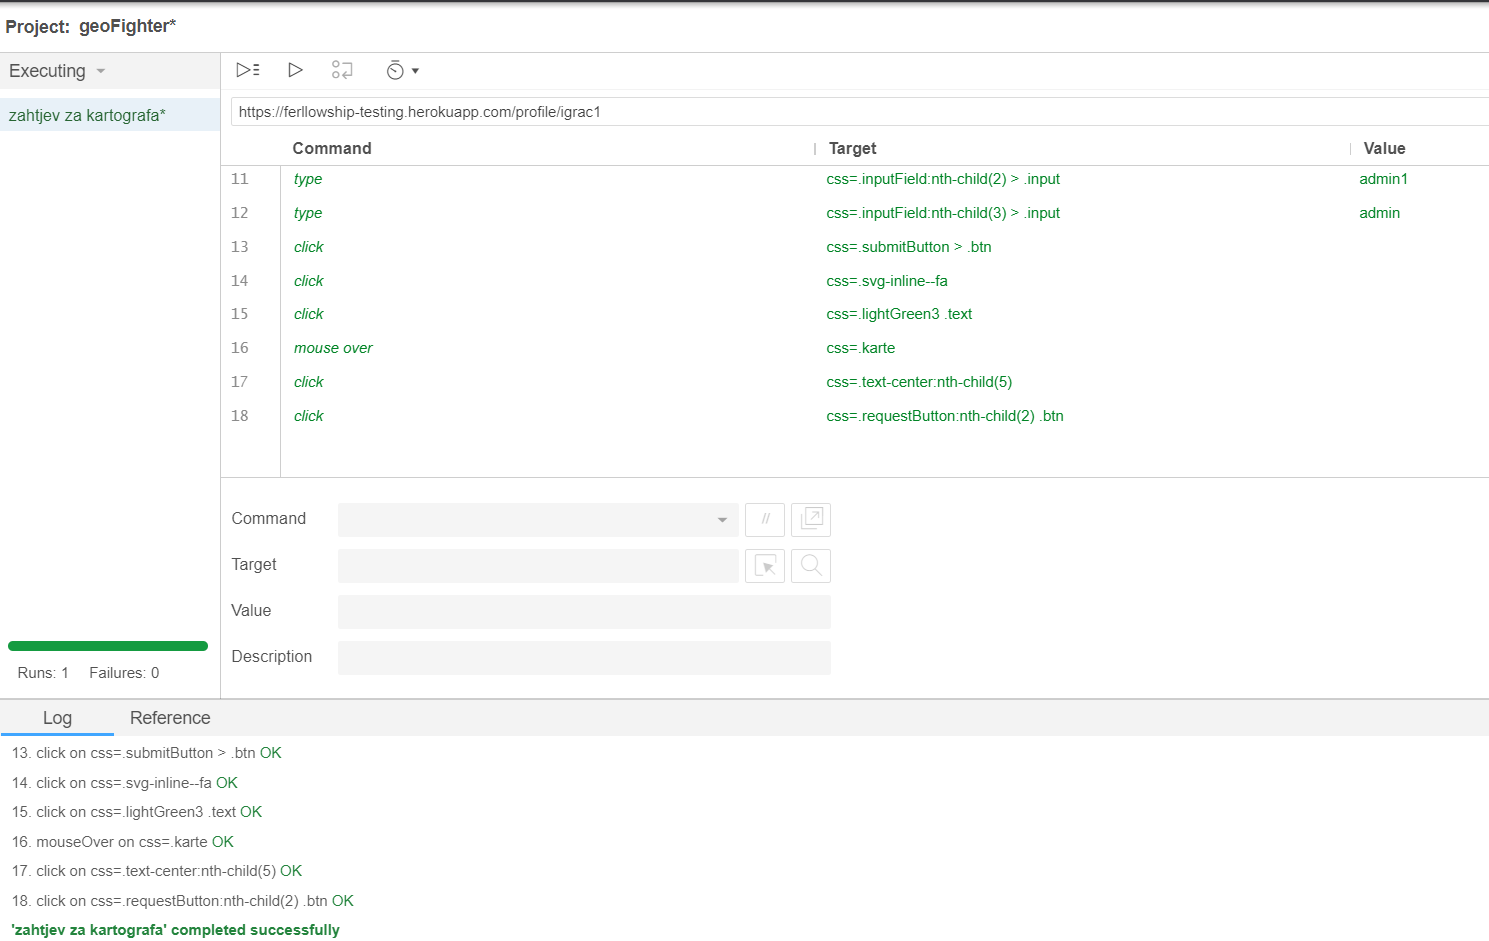
\includegraphics[width=\textwidth]{slike/SeleniumIDE_test2} 
						\centering
						\caption{Selenium IDE, ispitivanje zahtjeva za kartografa}
						\label{}
					\end{figure}
				
				
			\eject 
		
		
		\section{Dijagram razmještaja}
			
			%\textbf{\textit{dio 2. revizije}}
			
			 %\textit{Potrebno je umetnuti \textbf{specifikacijski} dijagram razmještaja i opisati ga. Moguće je umjesto specifikacijskog dijagrama razmještaja umetnuti dijagram razmještaja instanci, pod uvjetom da taj dijagram bolje opisuje neki važniji dio sustava.}
			
			{Dijagrami razmještaja (engl. deployment diagrams) opisuju topologiju skopovlja i programsku potporu koja se koristi u implementaciji sustava u njegovom radnom i produkcijskom okruženju. Dijagram razmještaja prikazuje razvijene aplikacije. Na poslužiteljskom računalu nalaze se web poslužitelj, poslužitelj baze podataka te poslužitelji Cloudinary i OSRM. Kako bi pristupili web aplikaciji, klijenti koriste web preglednik. Razmjena podataka između korisnika (igrač, kartograf, admin) i poslužitelja odvija se korištenjem HTTP protokola.}
			\begin{figure}[H]
				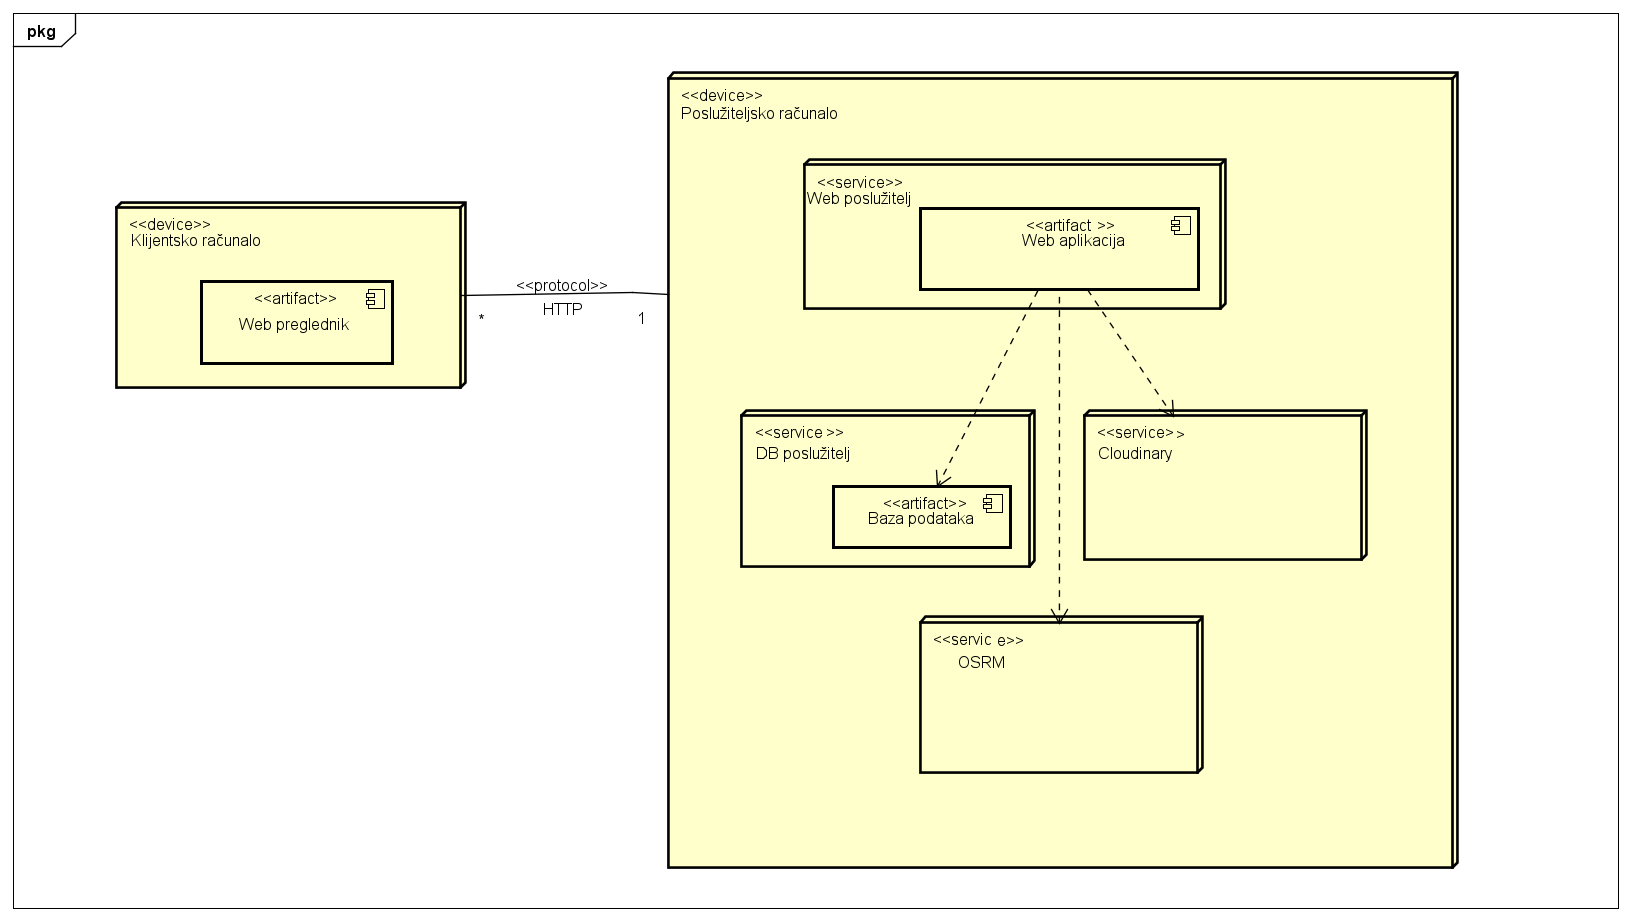
\includegraphics[width=\textwidth]{dijagrami/dijagram_razmjestaja} 
				\centering
				\caption{Dijagram razmještaja}
				\label{}
			\end{figure}
			\eject 
		
		\section{Upute za puštanje u pogon}
		
			\subsubsection{Uvod}
		
			{Aplikaciju je moguće lokalno pokrenuti tako da koristi H2 \textit{in-memory} poslužitelj baze podatka ili PostgreSQL poslužitelj. Najprije je opisan postupak instalacije i konfiguracije PostgreSQL poslužitelja. Ti koraci mogu se preskočiti jer su nakon toga dane upute za pokretanje pomoću \textit{docker-compose} skripte, čime je cijeli postupak značajno ubrzan i olakšan. Nakon toga opisan je način pokretanja Spring Boot aplikacije (\textit{backend} dio) i React aplikacije (\textit{frontend} dio.)}
			
			\subsubsection{Instalacija PostgreSQL poslužitelja baze podataka}
		
			 {Potrebno je preuzeti PostgreSQL bazu podataka za odabrani operacijski sustav. U ovisnosti o operacijskom sustavu, potrebno je provesti standardnu instalaciju.}
			 
 			\subsubsection{Konfiguracija PostgreSQL poslužitelja baze podataka}
			 
			 {Poslužitelj baze podataka treba biti namješten da koristi port 5432. Potrebno je postaviti korisnika \texttt{postgres} s lozinkom \texttt{root}. Također treba pripremiti praznu bazu podataka naziva \texttt{geofighter\_db}. Alternativni način postavljanja uključuje promjenu očekivanih parametara u datoteci \textit{application-pg.properties} koja se nalazi u direktoriju \texttt{backend/src/main/resources}.}
			
 			\subsubsection{Pokretanje pomoću \textit{docker-compose.yml} skripte}
			
			{U slučaju korištenja usluge \textit{Docker}, ovo je najjednostaviji način pokretanja PostgreSQL poslužitelja baze podataka. Iz komandne linije potrebno je pozicionirati se u direktorij \textit{backend} i pokrenuti naredbu \texttt{docker-compose up}. Svi potrebni parametri PostgreSQL poslužitelja bit će postavljeni na vrijednosti koje aplikacija očekuje.}
			
 			\subsubsection{Pokretanje Spring Boot aplikacije}
			
			{Za pokretanje Spring Boot aplikacije potrebno je, iz komandne linije, smjestiti se u direktorij \textit{backend} i pokrenuti naredbu \texttt{mvnw spring-boot:run -Dspring-boot.run.profiles=<profil>} (Windows) ili \texttt{./mvnw spring-boot:run -Dspring-boot.run.profiles=<profil>} (Linux). Odabrani profil može biti \texttt{pg} (PostgreSQL) ili \texttt{h2} (H2), ovisno o preferiranom poslužitelju. Ako se koristi profil \texttt{pg}, potrebno je najprije provesti ranije navedene korake za postavljanje PostgreSQL poslužitelja. Za profil \texttt{h2} nije ništa potrebno namještati.} 
			
			{Ako navedene naredbe za postavljanje profila ne rade, valja pokušati s \texttt{mvnw spring-boot:run -Dspring.profiles.active=<profil>} (Windows) ili \texttt{./mvnw spring-boot:run -Dspring.profiles.active=<profil>} (Linux). Profili pri tome poprimaju istu vrijednosti (\texttt{pg} ili \texttt{h2}).} 
			
			{Aplikacija će nakon pokretanja biti dostupna na portu 8080, a baza podataka će inicijalno biti popunjena podatcima zadanima u \texttt{data-<profil>.sql} skripti, pri čemu je profil \texttt{pg} ili \texttt{h2}.}
			
			{Kako bi se aplikacija mogla ispravno koristiti, potrebno je postaviti očekivane varijable okruženja. To su: EMAIL, EMAIL\_PASSWORD i CLOUDINARY\_URL. Varijable EMAIL i EMAIL\_PASSWORD predstavljaju podatke e-mail računa koji se koristi za slanje e-mail potvrde igračima koji su se tek registrirali. Varijabla CLOUDINARY\_URL je personalizirana veza na vanjsku uslugu \textit{Cloudinary} na koju se pohranjuju slike.}
			
 			\subsubsection{Pokretanje React aplikacije}
			
			{Za pokretanje React aplikacije potrebno je instalirati okruženje \textit{Node.js}, zajedno s upraviteljem paketa \textit{npm}. Prije pokretanja React aplikacije potrebno je napraviti prethodni korak (pokretanje Spring Boot aplikacije). Zatim je potrebno pozicionirati se u direktorij \textit{frontend} i najprije pokrenuti naredbu \texttt{npm install}, a zatim \texttt{npm start}. Time će se aplikacija postati dostupna na portu 3000, a automatski će se otvoriti \texttt{localhost:3000} u prozoru zadano postavljenog web preglednika.}
			
			\eject 